% The commands are as follows:
%
%  1)  PDFLaTex File.tex
%  2)  BibTex File
%  3)  PDFLaTex File.tex
%  4)  PDFLaTex File.tex
%
\documentclass[11pt, a4paper]{article}

\usepackage[affil-it]{authblk}% Same as APS affiliation
\usepackage{natbib}% Use with BibTex
\usepackage{graphicx}% Include figure files
\usepackage{amsmath}% Include math style
\usepackage{amsfonts}% Include font style
\usepackage{amssymb}% Include symbol symbols
\usepackage{dcolumn}% Align table columns on decimal point
\usepackage{bm}% Bold math
\usepackage{url}% Use urls
%\usepackage{hyperref}% add hypertext capabilities
%\usepackage[mathlines]{lineno}% Enable numbering of text and display math
\pagestyle{plain}
\renewcommand\harvardyearleft{\unskip, }
\renewcommand\harvardyearright[1]{.}
%\usepackage[showframe,%Uncomment any one of the following lines to test 
%scale=0.7, marginratio={1:1, 2:3}, ignoreall,% default settings
%text={7in,10in},centering,
%margin=1.5in,
%total={6.5in,8.75in}, top=1.2in, left=0.9in, includefoot,
%hmargin={1cm,0.8in},
%]{geometry}


\begin{document}

\title{Summary Report}

\author{Gerwyn Jones}
\affil{Physics Department, Cardiff University.}

\date{\today}

\maketitle

%%%%%%%%%%%%%%%%%%%% ABSTRACT %%%%%%%%%%%%%%%%%%

\begin{abstract}

Talk about Abstract

\end{abstract}


%%%%%%%%%%%%%%%%%%%% INTRODUCTION %%%%%%%%%%%%%%%%%%


\section{\label{sec:level1} Introduction }

Talk about Introduction

\cite{Bartelli.Motta.2016}

\subsection{Maths}
\label{sec:maths} % used for referring to this section from elsewhere

Simple mathematics can be inserted into the flow of the text e.g. $2\times3=6$
or $v=220$\,km\,s$^{-1}$, but more complicated expressions should be entered
as a numbered equation:

\begin{equation}
    x=\frac{-b\pm\sqrt{b^2-4ac}}{2a}.
	\label{eq:quadratic}
\end{equation}

Refer back to them as e.g. equation~(\ref{eq:quadratic}).

%%%%%%%%%%%%%%%%%%%% CONCLUSION %%%%%%%%%%%%%%%%%%


\section{\label{sec:level1} Conclusion }

Talk about Conclusion
\\
Figures are referred to as e.g. Fig.~\ref{fig:example_figure}

% Example figure
\begin{figure}[h]
	% To include a figure from a file named example.*
	% Allowable file formats are eps or ps if compiling using latex
	% or pdf, png, jpg if compiling using pdflatex
	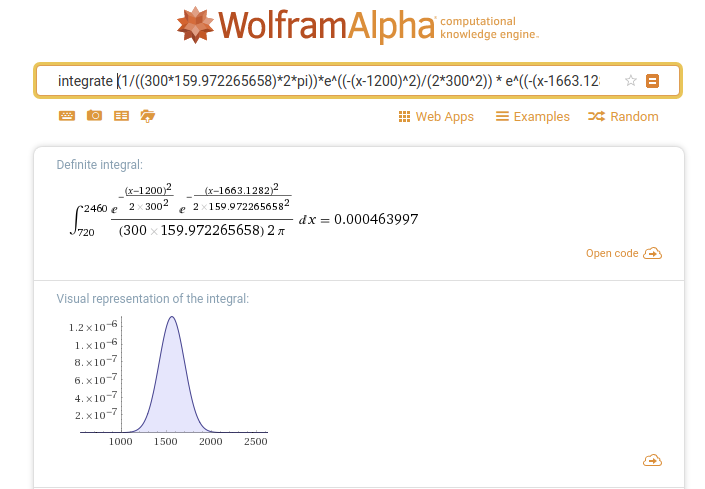
\includegraphics[width=\columnwidth]{Example1}
    \caption{This is an example figure. Captions appear below each figure.
	Give enough detail for the reader to understand what they're looking at,
	but leave detailed discussion to the main body of the text.}
    \label{fig:example_figure}
\end{figure}


%%%%%%%%%%%%%%%%%%%% REFERENCES %%%%%%%%%%%%%%%%%%

\bibliographystyle{myhavard}
\bibliography{BibTex_Entries}

\end{document}
